\documentclass[twoside,b5paper,10pt]{article}
\usepackage{AUTstyle}


\title{Knowledge base population using natural language inference }
\author{Recski Gabor \and Kovacs Adam}

\institution{Department of Automation and Applied Informatics \\
Budapest University of Technology and Economics}

\email{\{recski,adaam.ko\}@aut.bme.hu}

\headerTitle{Knowledge base population \dots}
\headerAuthor{Recski Gabor and Kovacs Adam}



\begin{document}
\makeAutStyleTitle


\begin{abstract}
  We present a set of pilot experiments for augmenting a generic, open-domain 
  knowledge base using a graph-based lexical ontology of English and simple
  inference rules. WikiData knowledge base contains facts encoded as relation
  triplets, such as author(George Orwell, 1984), based on which naive
  speakers can easily establish additional facts such as that George Orwell is a
  person and 1984 is some written work, most likely a book. To automate this type
  of inference we need models of lexical semantics that are more explicit than
  the distributional models commonly used in computational semantics. The 4lang
  library provides tools for building concept graph representations of the
  semantics of natural language text, its module \verb|dict_to_4lang| processes entries
  of monolingual dictionaries to build 4lang-style definition graphs of virtually
  any English word. The representation of "author" will likely contain edges
  corresponding to facts such as \verb|IS_A|(author, person) and write(author, book).
  We define simple templates that use these representations for inference over
  WiktData facts; preliminary evaluation on small samples suggests our method's
  precision to be in the $0.7$-$0.8$ range.
\end{abstract}


\begin{keywords}
semantics; inference; natural language processing;
\end{keywords}

\section{Introduction}
\label{sec:Introdu}

In this paper I present a way of matching \verb|WikiData| relations with arguments of 
\verb|4lang| definitions. The \verb|dict_to_4lang| tool automatically builds graphs from longman dictionary definitions. 
The full pipeline is available for download under an MIT license at \verb|https://github.com/adaamko/4lang|.
\verb|WikiData| is a publicly available knowledge base and we can make triplets out of it in the form of \verb|predicate(argument1, argument2)|. 
If we can make an assumption that these arguments corresponds to each other and a set of patterns can be applied to them, then we can  convert a large amount of information from WikiData to the 4lang format and combine the two knowledge.

\section{Combine WikiData and 4lang}
\label{sec:Combine WikiData and 4lang}
The 4lang pipeline maps the output of the Standford dependency parser to subgraphs representing the words of each definition.  
For example \texttt{father} is defined in longman as \texttt{male parent}. 
The \verb|dict_to_4lang| tool uses this definition to build a 4lang graph seen in \figurename~\ref{fig:father}(default). 
If we have a triplet coming from the WikiData knowledge base such as father(Az-Zahir Ghazi, Saladin) and we are ready to make 
an assumption that the second argument corresponds with the only IS A relation of out graph, then we can combine the fact with 
the longman definiton to obtain a new graph shown in Figure \figurename~\ref{fig:father}(expanded). We have a new machine a IS A relation, the 
\texttt{Saladin}~$\xrightarrow0$~\texttt{male} 0 edge that wasnt present before. We can see that we could obtain a completely 
new information which was unknown from the definition graph and from the Wikidata alone, and could only be present from the combination
of the two. If we want to build 4lang graphs automatically from WikiData, we will require a method for matching these relations, as in the case above. 
The result will have to be reviewed, and only the reasonable ones have to be selected. If we can apply patterns to these triplets and definitons, 
we can have a large amount of information retrieved from the combination of the two.

\begin{figure}[htb]
  \vspace{3pt}
  \centerline{
  \hbox{
  \hspace{0.0in}
        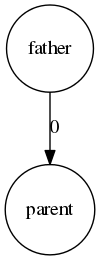
\includegraphics[scale=0.5]{Figure/father.png}
        \hspace{0.1\columnwidth}
        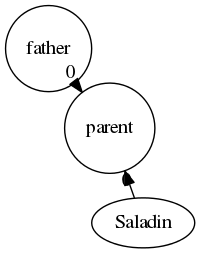
\includegraphics[scale=0.5]{Figure/fathernew.png}
    }
  }
  \vspace{3pt}
  \hbox{\hspace{0.23\columnwidth} (default) \hspace{0.3\columnwidth} (expanded)}
  \caption{ (default) father definition (expanded) father with gained information}
  \label{fig:father}
\end{figure}

\section{Methods}
\label{sec:Methods}
From the examination of the WikiData triplets, we can have a suspicion that if we say have a 0 edge in our definition graph \texttt{predicate}~$\xrightarrow0$~\texttt{X} 
then in our new graph coming from the combination of the WikiData and the 4lang graph, a machine looks like \texttt{arg2}~$\xrightarrow0$~\texttt{X} most likely 
going to have a place. And if we have an edge \texttt{predicate}~$\xrightarrow2$~\texttt{X} in our original graph, then we will have an  edge \texttt{arg1}~$\xrightarrow0$~\texttt{X} 
in the newly constructed graph. As we can see in \figurename~\ref{fig:creator}(default) and \figurename~\ref{fig:creator}(expanded) new machines appeared such as \texttt{OpenCart}~$\xrightarrow0$~\texttt{thing} and 
\texttt{Daniel Kerr}~$\xrightarrow0$~\texttt{made} both of these appear to be valid information thanks to out pattern. Of course this is an ideal situation, this will not be always the case, 
there are many factors to be considered, when we apply these patterns to out data. We have to take into account the fact, that the triplets coming from the WikiData are not always going to 
be valid information. This case can be seen in \figurename~\ref{fig:tributary}(default) and \figurename~\ref{fig:tributary}(expanded), where one of the arguments of a WikiData triplet was \texttt{novalue}, 
so the edge created from the triplet does not holds any information. There are cases, when the originally created graph is not completely parsed right from the definition. \texttt{flag} is 
definition in longman is: \texttt {piece of cloth with a coloured pattern or picture on it that represents a country}. The definition graph built from this definition is in \figurename~\ref{fig:flag}. 
The machine \texttt{flag}~$\xrightarrow0$~\texttt{piece} obviously does not contain valid information, so the triplet flag(Belgium,flag of Belgium) with our current pattern would not add additional 
information to it. Our parser does not handle when there are multiple choices in a definition. For example longman defines employer \texttt{a person, company, or organization that employs people}. 
The graph constructed in \figurename~\ref{fig:employer}(default) and \figurename~\ref{fig:employer}(expanded). We have an IS a edge \texttt{Central Intelligence Agency}~$\xrightarrow0$~\texttt{person} which we can presume is not a valid assumption, 
it would be rather a company. The next case, where out pattern can fail is when the WikiData and the longman has different definition of a word, it was the case when we examined the word Developer, which definition in 
longman was \texttt{a person or company that makes money by buying land and then building houses, factories etc on it} but the triplet in WikiData assumed it was a Software Developer as we can see Developer(De Blob, Blue Tongue Entertainment).

\begin{figure}[htb]
  \vspace{3pt}
  \centerline{
  \hbox{
  \hspace{0.0in}
        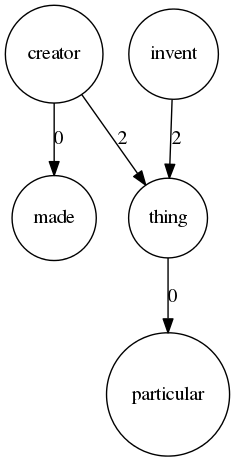
\includegraphics[scale=0.5]{Figure/creator.png}
        \hspace{0.1\columnwidth}
        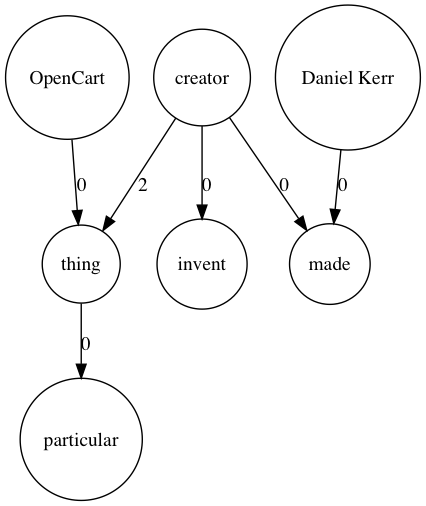
\includegraphics[scale=0.5]{Figure/creatornew.png}
    }
  }
  \vspace{3pt}
  \hbox{\hspace{0.13\columnwidth} (default) \hspace{0.3\columnwidth} (expanded)}
  \caption{ (default) creator definition (expanded) creator with gained information}
  \label{fig:creator}
\end{figure}

\begin{figure}[htb]
  \vspace{3pt}
  \centerline{
  \hbox{
  \hspace{0.0in}
        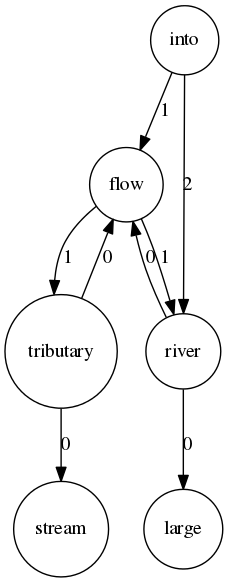
\includegraphics[scale=0.5]{Figure/tributary.png}
        \hspace{0.1\columnwidth}
        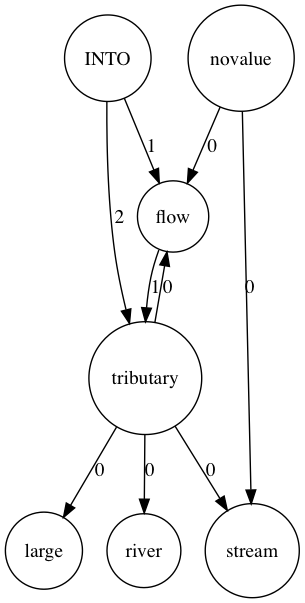
\includegraphics[scale=0.5]{Figure/tributarynew.png}
    }
  }
  \vspace{3pt}
  \hbox{\hspace{0.13\columnwidth} (default) \hspace{0.3\columnwidth} (expanded)}
  \caption{ (default) tributary definition (expanded) tributary with gained information}
  \label{fig:tributary}
\end{figure}

\begin{figure}[htb]
  \centerline{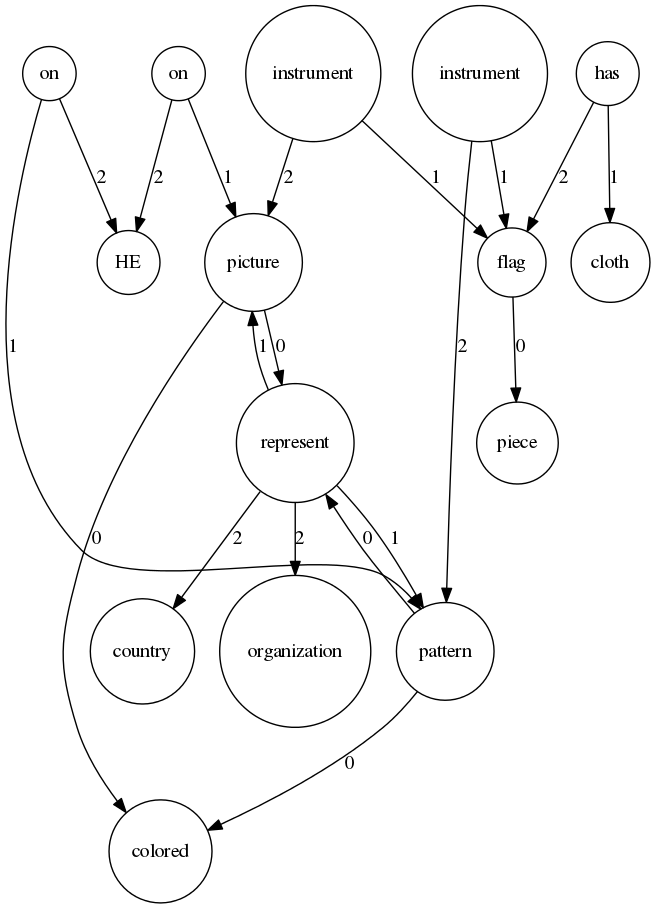
\includegraphics[scale=0.3]{Figure/flag.png}}
  \caption{Flag definition}
  \label{fig:flag}
 \end{figure}

 \begin{figure}[htb]
  \vspace{3pt}
  \centerline{
  \hbox{
  \hspace{0.0in}
        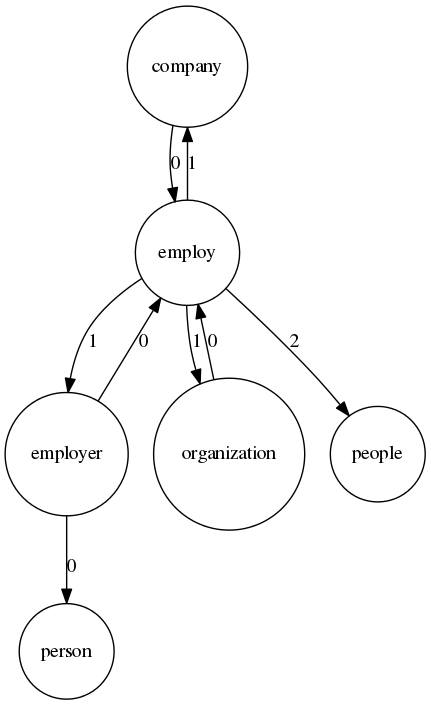
\includegraphics[scale=0.4]{Figure/employer.png}
        \hspace{0.1\columnwidth}
        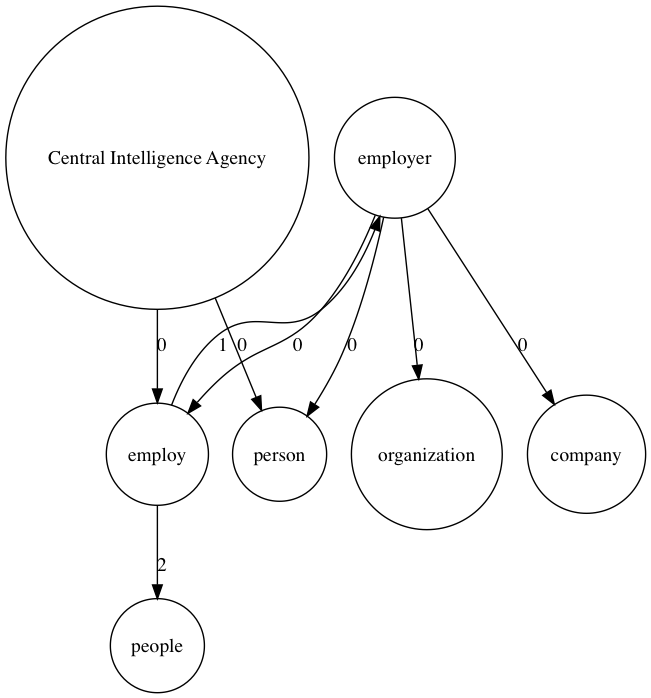
\includegraphics[scale=0.4]{Figure/employernew.png}
    }
  }
  \vspace{3pt}
  \hbox{\hspace{0.13\columnwidth} (default) \hspace{0.3\columnwidth} (expanded)}
  \caption{ (default) employer definition (expanded) employer with gained information}
  \label{fig:employer}
\end{figure}

\section{Testing and Conclusions}
\label{sec:Testing}
Knowing these facts we can make a few assumptions for increasing the possibility of the additional information's correctness. 
We can separate the two types of method we introduced earlier and inspect each one individually. Our initial thought was to design an algorithm
that can identify the correct edges. For example, when there is only one $0$ or $2$ type edge in the definition
graph or there is no ingoing edge to the predicate, there is a higher chance that the additional information that we gained by the mapping will be correct.
Using these techniques we performed quantitative evaluation by manually inspecting a small output sample, that contained these kind of assumptions.
We found out, that we have a higher success rate by closing out those automatically that we think will give us false information such as invalid information
in the WikiData dataset or when there are multiple choices in the longman definition and we didn't select the ones where there was no edge or node found. By examinating the sample size of 3000 graphs, our algorithm for edge type 0
closed out 1252 of them and for edge type 2 it closed out 2647. From the remaining ones, we manually chose 100 random ones, and we found that
77 of them were near perfect. From these informations, we can assume that using the methods explained, we can reach 77 percent success rate.
For gaining we could combine the algorithms designed for identifying the incorrect ones with the one choosing the right ones. 
This way from the remaining 1728 with type edge 0, our methods suggest that 1559 is correct, 899 out of it is because of the no ingoing edge rule and 660 is coming from the single zero edge rule.
With edge type 2 from the remaining 353 we think 220 is correct 55 of them is coming from the no ingoing edge, 37 because of the single edge rule and 128 containing both. 


\section{Bibliography}
\label{sec:bib}

You have to use the \verb|\makeAutBib| command for your
bibliography. The input parameter of the command is the comma
separated list of bib files without the extension. You can also find
a sample bib file on the Workshop's web site where also the style
file and this sample \LaTeX \ template are provided. You can cite
any of the entries of the bib files for example ~\cite{ han00mining}
or ~\cite{burdick01mafia}. The advantage of using bib files is that
only those bibliographies will appear in the References section that
are cited in the text \cite{proba}.

If you have any question related to writing your \LaTeX \ paper
please contact the chair of the conference(e-mail: aacs@aut.bme.hu).

You can submit your paper via the web page of the conference. The
submission of the papers will be opened soon.

\section*{Acknowledgments}
 { \small The author would like to express his thanks to Istv�n Vajk~\footnote{Please mention the name of your advisor in the
Acknowledgements section. } for his support as a scientific advisor.
This work has been supported by the \dots \footnote{Please mention
the institution or organization that has supported your research
work.} }

\makeAutBib{reni,itemsetmining}

\end{document}
